\subsection{Пайплайн работы сервиса}
У микросервиса есть свой пайплайн запуска некоторых процессов при активации хендлера.
Такой подход к программированию позволяет делать встраивание различных функциональностей по пути и масштабировать сервис вширь.
В данном разделе будет описан пайплайн работы сервиса для парсинга картинок.

Для начала сервис необходимо инициализировать различного рода переменными, которые содержат в себе секреты такие, как пароли.
Данная информация хранится в ENV переменных.

На рисунке~\ref{flags-func-add} изображен снипет кода, в котором написана функция, при помощи которой происходит забор всех необходимых секретов из yaml файла.
На рисунке~\ref{yaml-secret-add} представлен пример подобного yaml файла.

Далее происходит инициализация роутинга, после чего инициализируются объекты класса, которые выполняют всю работу.

Код всего парсинга начинается с пакета parser. Напомню, что схема всего проекта находится на рисунке~\ref{clean-arch-add}.
Информация из parser, ответ которой являются ссылки, далее ведет к пакету image-getter. Этот пакет начинает в асинхронном режиме скачивать все картинки.
Для обработки ошибок в асинхронном режиме, пришлось придумать систему, которая могла бы записать ошибки, если таковые были, а затем после окончания работы всех горутин сообщить о том, что где-то возникла ошибка.
На рисунке~\ref{err-controller-snippet} изображен пример кода, который выполняет вышеизложенную фукнцию.

\begin{figure}
    \begin{lstlisting}[language=go]
        // IsNul проверяет, что нет ошибок.
        // Если ошибки есть, то возвращает эти ошибки и, ВНИМАНИЕ, обнуляет массив ошибок.
        // После повторного вызова IsNul будет всегда возвращаться nil.
        func (e *ErrController) IsNul() []error {
            e.mx.Lock()
            defer e.mx.Unlock()

            if e.errors == nil {
                return nil
            }
            result := make([]error, len(e.errors))
            copy(result, e.errors)
            e.errors = nil
            return result
        }

        // PutError кладет ошибки в стэк ошибок для дальнейшей их обработки
        func (e *ErrController) PutError(err error) {
            e.mx.Lock()
            defer e.mx.Unlock()
            e.errors = append(e.errors, err)
        }
    \end{lstlisting}
    \caption{Пример кода с контролированием ошибок}
    \label{err-controller-snippet}
\end{figure}

Как видно, в данном коде присутствует мьютекс. Он нас сможет защитить от гонки.

После того, как файлы скачались в определенное место на диске, мы должны либо передать на выход хендлера байтовое представление готовых файлов.
Либо мы идем в пакет pdf-builder, где идет сбор всех картинок в один большой pdf.

На рисунке~\ref{pipeline-pic} изображен описанный выше пайплайн, где в фигурках диаграммы написаны названия пакетов.

\begin{figure}
    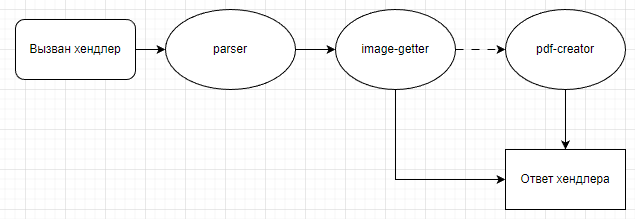
\includegraphics[scale=0.8]{imgs/pipeline}
    \caption{Диаграмма пайплайна}
    \label{pipeline-pic}
\end{figure}